\documentclass[a4paper,12pt]{article}
\usepackage[utf8]{inputenc}
\usepackage{geometry}
\geometry{top=2cm, bottom=2cm, left=2.5cm, right=2.5cm}
\usepackage{graphicx}
\usepackage{titlesec}
\usepackage{enumitem}
\usepackage{fancyhdr}
\usepackage{setspace}
\usepackage{todonotes}
\usepackage[normalem]{ulem}
\pagestyle{fancy}
\fancyhf{}
\rhead{Progetto Basi di Dati 2024-25}
\lhead{“FANTASANREMO”}
\cfoot{\thepage}

\titleformat{\section}{\normalfont\Large\bfseries}{\thesection.}{1em}{}
\titleformat{\subsection}{\normalfont\large\bfseries}{\thesubsection}{1em}{}

\begin{document}

\begin{center}
    {\LARGE \textbf{Progetto Basi di Dati 2024-25}}\\[.5cm]
    {\Large \textbf{“FANTASANREMO”}}\\[.5cm]
    {\Large \textbf{PARTE I}}\\[.8cm]
    Team 35\\[.3cm]
    Alessio Molinas 5339413\\
    Ettore Romano 5644926
\end{center}

\vspace{1cm}

\section{REQUISITI RISTRUTTURATI}
%[Riportare in questa sezione la specifica dei requisiti ristrutturata in modo da eliminare ambiguità, evidenziando eventuali modifiche effettuate rispetto alla specifica fornita]
Si richiede la progettazione e realizzazione di una base di dati a supporto della piattaforma social di FantaSanremo, un gioco di fantasia ispirato al Festival di Sanremo.

Il gioco consente agli utenti (che si registrano con nome e cognome, identificati dalla loro username) di creare e gestire squadre virtuali (alle quali attribuiscono un nome, identificate da un codice) di artisti (i cantanti) partecipanti, organizzandosi in leghe (alle quali viene assegnato un nome, identificate da un codice) per competere tra loro. I punteggi vengono assegnati in base alle performance degli artisti e all’applicazione di specifici bonus e malus (con descrizione, valore, tipologia bonus, identificati da un codice). La base di dati dovrà permettere la gestione strategica delle squadre, l’organizzazione delle leghe e il tracciamento in tempo reale dei punteggi durante il Festival.

Un primo aspetto fondamentale riguarda la gestione del Festival stesso. È necessario memorizzare le informazioni relative agli artisti in gara, inclusi dettagli come nome, biografia, genere musicale, provenienza (luogo e data di nascita) e partecipazioni passate. Per ogni artista, sarà importante associare i brani eseguiti, registrandone titolo, autori, compositori, durata e genere musicale. E' inoltre importante sapere chi dirige il brano. Ogni esibizione dovrà essere collegata a una specifica serata del Festival (le serate vengono considerate come dei contenitori), con indicazione dell’ordine di esibizione, dell’orario e di eventuali altri dettagli rilevanti.
Inoltre, il sistema dovrà raccogliere e conservare i voti assegnati dai diversi organi di giuria e dal pubblico, consentendo così di monitorare l’andamento della competizione e aggiornare la classifica del Festival in base ai risultati (tipologia voto, data ed ora, identificato da un codice progressivo).

Parallelamente, la base di dati dovrà supportare le dinamiche del gioco FantaSanremo. Gli utenti dovranno registrarsi con un nome univoco (username che di fatto corrisponde all'indirizzo e-mail) e fornire informazioni personali essenziali (nome, cognome). Ogni utente avrà la possibilità di creare squadre, rispettando un budget di crediti virtuali 100 (baudi), con cui selezionare sette artisti tra quelli in gara. La formazione prevede cinque titolari, due riserve e un capitano scelto tra i titolari. Sarà possibile iscrivere e modificare la squadra entro una data limite, con la possibilità di riorganizzare la formazione giornalmente durante la settimana del Festival, rispettando precise fasce orarie. I punteggi vengono assegnati in base a un regolamento che prevede l’attribuzione di bonus e malus agli artisti in base alle loro performance e ad altri criteri specificati (sono censiti con descrizione, tipo, valore (positivo/negativo) ed  indentificati da un codice).

Gli artisti schierati tra i titolari contribuiscono al punteggio totale della squadra con tutti i bonus e malus accumulati, mentre quelli tra le riserve influenzano il punteggio solo con bonus e malus di tipo extra. Il capitano ottiene un trattamento speciale per alcuni bonus, con punteggi raddoppiati in determinate circostanze. Il gioco si articola in leghe (con nome, tipo visibilità), che permettono agli utenti di sfidarsi in campionati separati. Le leghe possono essere pubbliche, private o segrete, con diverse modalità di accesso e visibilità. Ogni lega ha un nome personalizzabile e può essere amministrata da un proprietario (l’utente che l’ha creata) e da eventuali amministratori delegati.
Il proprietario e gli amministratori hanno il compito di gestire la lega e approvare le richieste di iscrizione nelle leghe private e segrete, ma non possono intervenire sui punteggi assegnati agli artisti, che vengono determinati secondo il regolamento ufficiale del gioco. Ogni utente può creare un numero limitato di leghe e partecipare a un massimo di venticinque leghe contemporaneamente. Ogni lega consente a ciascun partecipante di iscrivere una sola squadra, e tutte le squadre sono automaticamente iscritte anche al Campionato Mondiale dell’edizione in corso del Festival (una lega pubblica). Durante lo svolgimento del Festival, il sistema dovrà calcolare e aggiornare i punteggi delle squadre al termine di ogni serata, aggiornando di conseguenza la classifica delle leghe e quella generale del Campionato Mondiale. Al termine della competizione, la squadra con il punteggio più alto all’interno di ciascuna lega sarà dichiarata vincitrice.


\section{PROGETTO CONCETTUALE}
\subsection{Schema Entity Relationship}
%[Riportare in questa sezione il diagramma ER, indicando anche il tipo delle gerarchie di generalizzazione]
\begin{center}
	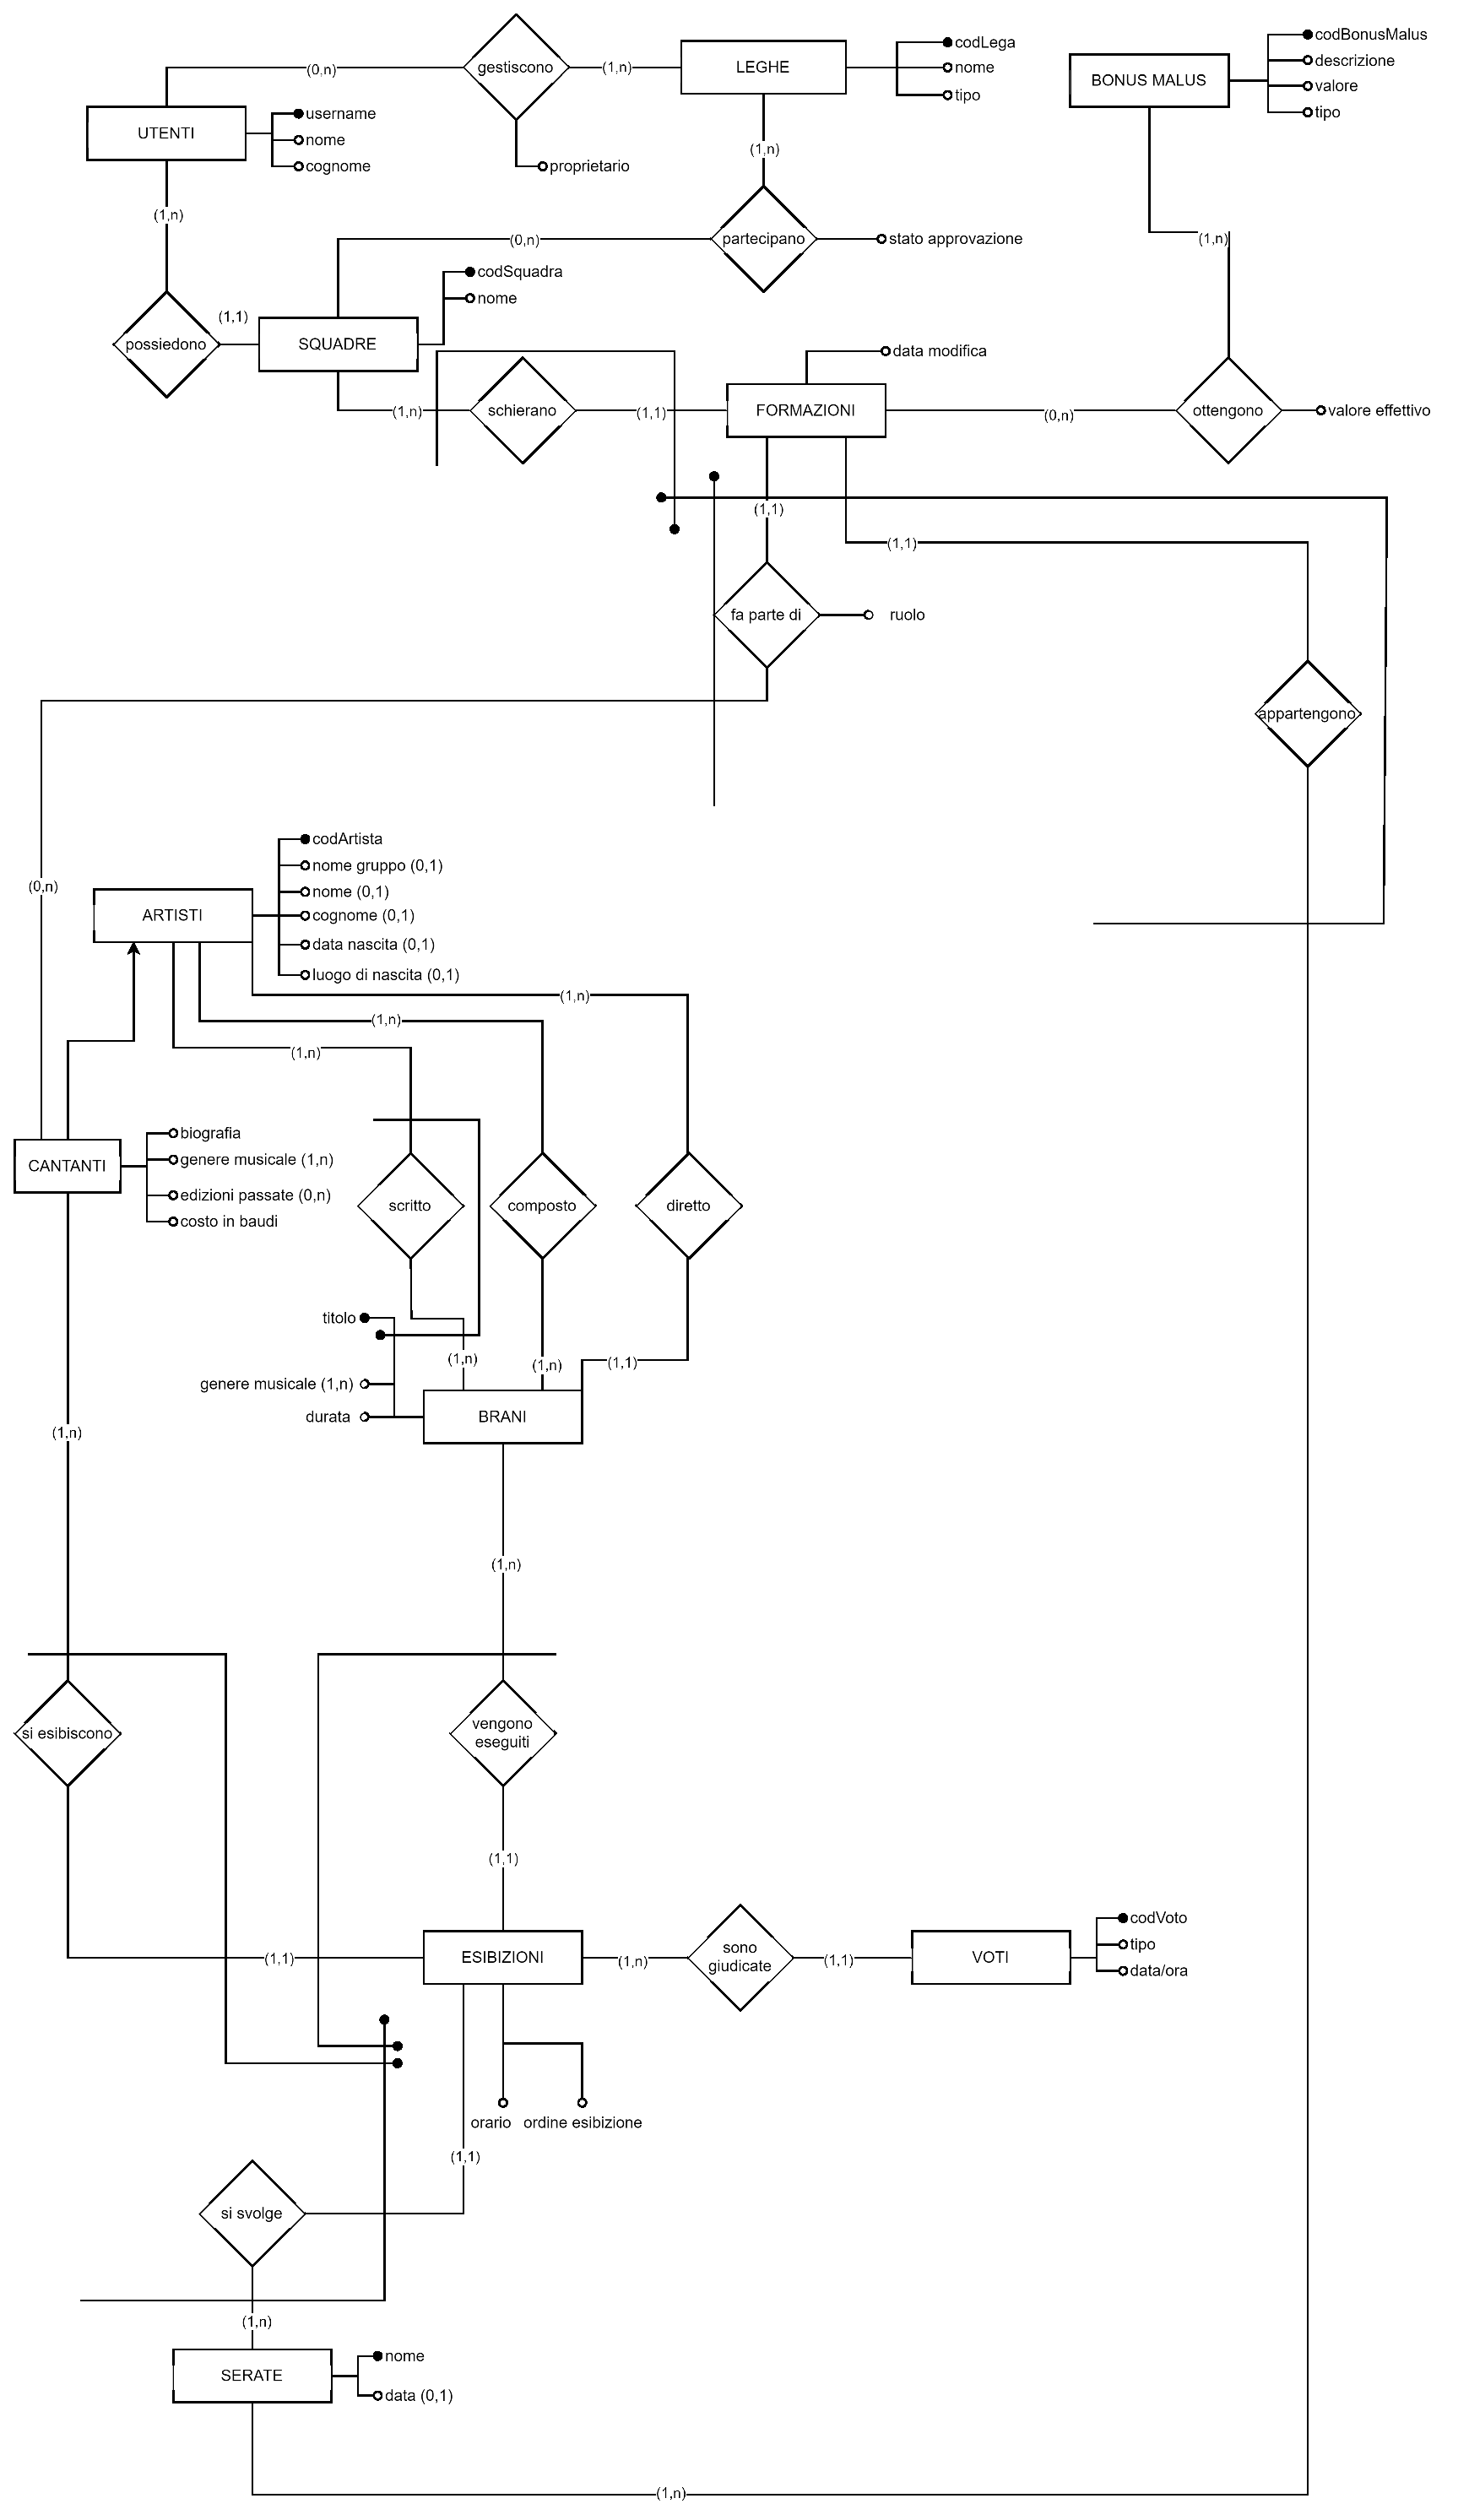
\includegraphics[width=0.8\textwidth]{schema_ER.eps}
\end{center}

% tabella entità padre-figlie
\begin{table}[h!]
	\centering
	\begin{tabular}{|c|c|p{5cm}|p{5cm}|}
		\hline
		\textbf{Entità padre} & \textbf{Entità figlia} & \textbf{Tipologia} & \textbf{Attributi aggiuntivi} \\ \hline
		artisti & cantanti & associazione di sottoinsieme: parziale ed esclusiva & biografia, genere musicale, edizioni passate, costo in baudi \\ \hline
	\end{tabular}
	\caption{Tipo gerarchie di generalizzazione}
\end{table}

\subsection{Dizionario Dati – Domini degli Attributi}
%[Specificare i domini degli attributi non ovvi]
	\begin{itemize}
		\item \textbf{(tipo, voti)} = tipo\_voto
		\begin{itemize}
			\item tipo\_voto = \{televoto, giuria\_stampa, giuria\_radio\}
		\end{itemize}
		
		\item \textbf{(tipo, leghe)} = tipo\_lega
		\begin{itemize}
			\item tipo\_lega = \{pubblica, privata, segreta\}
		\end{itemize}
		
		\item \textbf{(username, utenti)} = stringa
		
		\item \textbf{(proprietario, gestiscono)} = bool
		
		\item \textbf{(stato approvazione, partecipano)} = tipo\_approvazione
		\begin{itemize}
			\item tipo\_approvazione = \{IN\_APPROVAZIONE, RIFIUTATA, APPROVATA\}
		\end{itemize}
		
		\item \textbf{(tipo, bonus malus)} = tipo\_bonusmalus
		\begin{itemize}
			\item tipo\_bonusmalus = \{EXTRA, STANDARD\}
		\end{itemize}
		
		\item \textbf{(valore, bonus malus)} = real (può essere negativo per i malus)
		
		\item \textbf{(ruolo, compone)} = ruolo\_compone
		\begin{itemize}
			\item ruolo\_compone = \{CAPITANO, TITOLARE, RISERVA\}
		\end{itemize}
		
		\item \textbf{(durata, brani)} = real (secondi durata brano)
	\end{itemize}
\newpage
\subsection{Vincoli Non Esprimibili nel Diagramma}
	\begin{table}[h!]
	    \centering
	    \begin{tabular}{|c|c|p{6.5cm}|}
	        \hline
	        \textbf{Numero Vincolo} & \textbf{Entità e/o Associazioni Coinvolte} & \textbf{Vincolo in Linguaggio Naturale} \\ \hline
	        1 & utenti, squadre, leghe, partecipano & Un utente con le proprie squadre non può partecipare a più di 25 leghe \\ \hline
	        2 & utenti, formazioni, squadre & Ogni utente, per ciascuna formazione di una squadra, ha a disposizione 100 baudi \\ \hline
	       	3 & squadre, formazioni, serate & Una squadra, per ciascuna serata, può avere al massimo 7 partecipanti alla formazione (se durante la giornata la formazione cambia più volte nella fascia oraria concessa, sarà sovrascritta e aggiornata la data di modifica) \\ \hline
	        4 & squadre, formazioni, cantanti & Per ciascuna data, per ciascuna squadra, potremo avere al massimo 4 titolari, 2 riserve, 1 capitano all'interno della formazione \\ \hline
	        5 & leghe, partecipano & Se la tipologia di lega è pubblica, il tipo di approvazione dell'associazione 'partecipano' è valorizzato ad "APPROVATA". \\ \hline
	        6 & artisti, scritto, composto, diretto & Se l'artista è un gruppo (attributo 'nome gruppo' valorizzato), non potrà scrivere, comporre o dirigere brani \\ \hline
	        7 & artisti & Se l'artista ha valorizzato l'attributo 'nome gruppo', non potrà avere valorizzati 'nome', 'cognome', 'data nascita' e 'luogo nascita', e viceversa  \\ \hline
	    \end{tabular}
	    \caption{Vincoli Non Esprimibili nel Diagramma ER}
	\end{table}
\subsection{Commenti e Scelte Effettuate}
Come scelta implementativa abbiamo deciso di rappresentare nel database "il gruppo" come un oggetto unico e non come insieme di persone che lo compongono. Dal nostro punto di vista, il gruppo partecipa alla gara e non i singoli membri. I brani non vengono scritti/composti/diretti da un gruppo, ma da artisti (che eventualmente potrebbero fare parte di un gruppo, ma non teniamo traccia di questo elemento). In breve, lo schema non vuole tenere in considerazione la composizione dei gruppi.

\newpage
\section{PROGETTO LOGICO}
\subsection{Schema ER Ristrutturato}
%[inserire qui il diagramma ER ristrutturato]
\begin{center}
	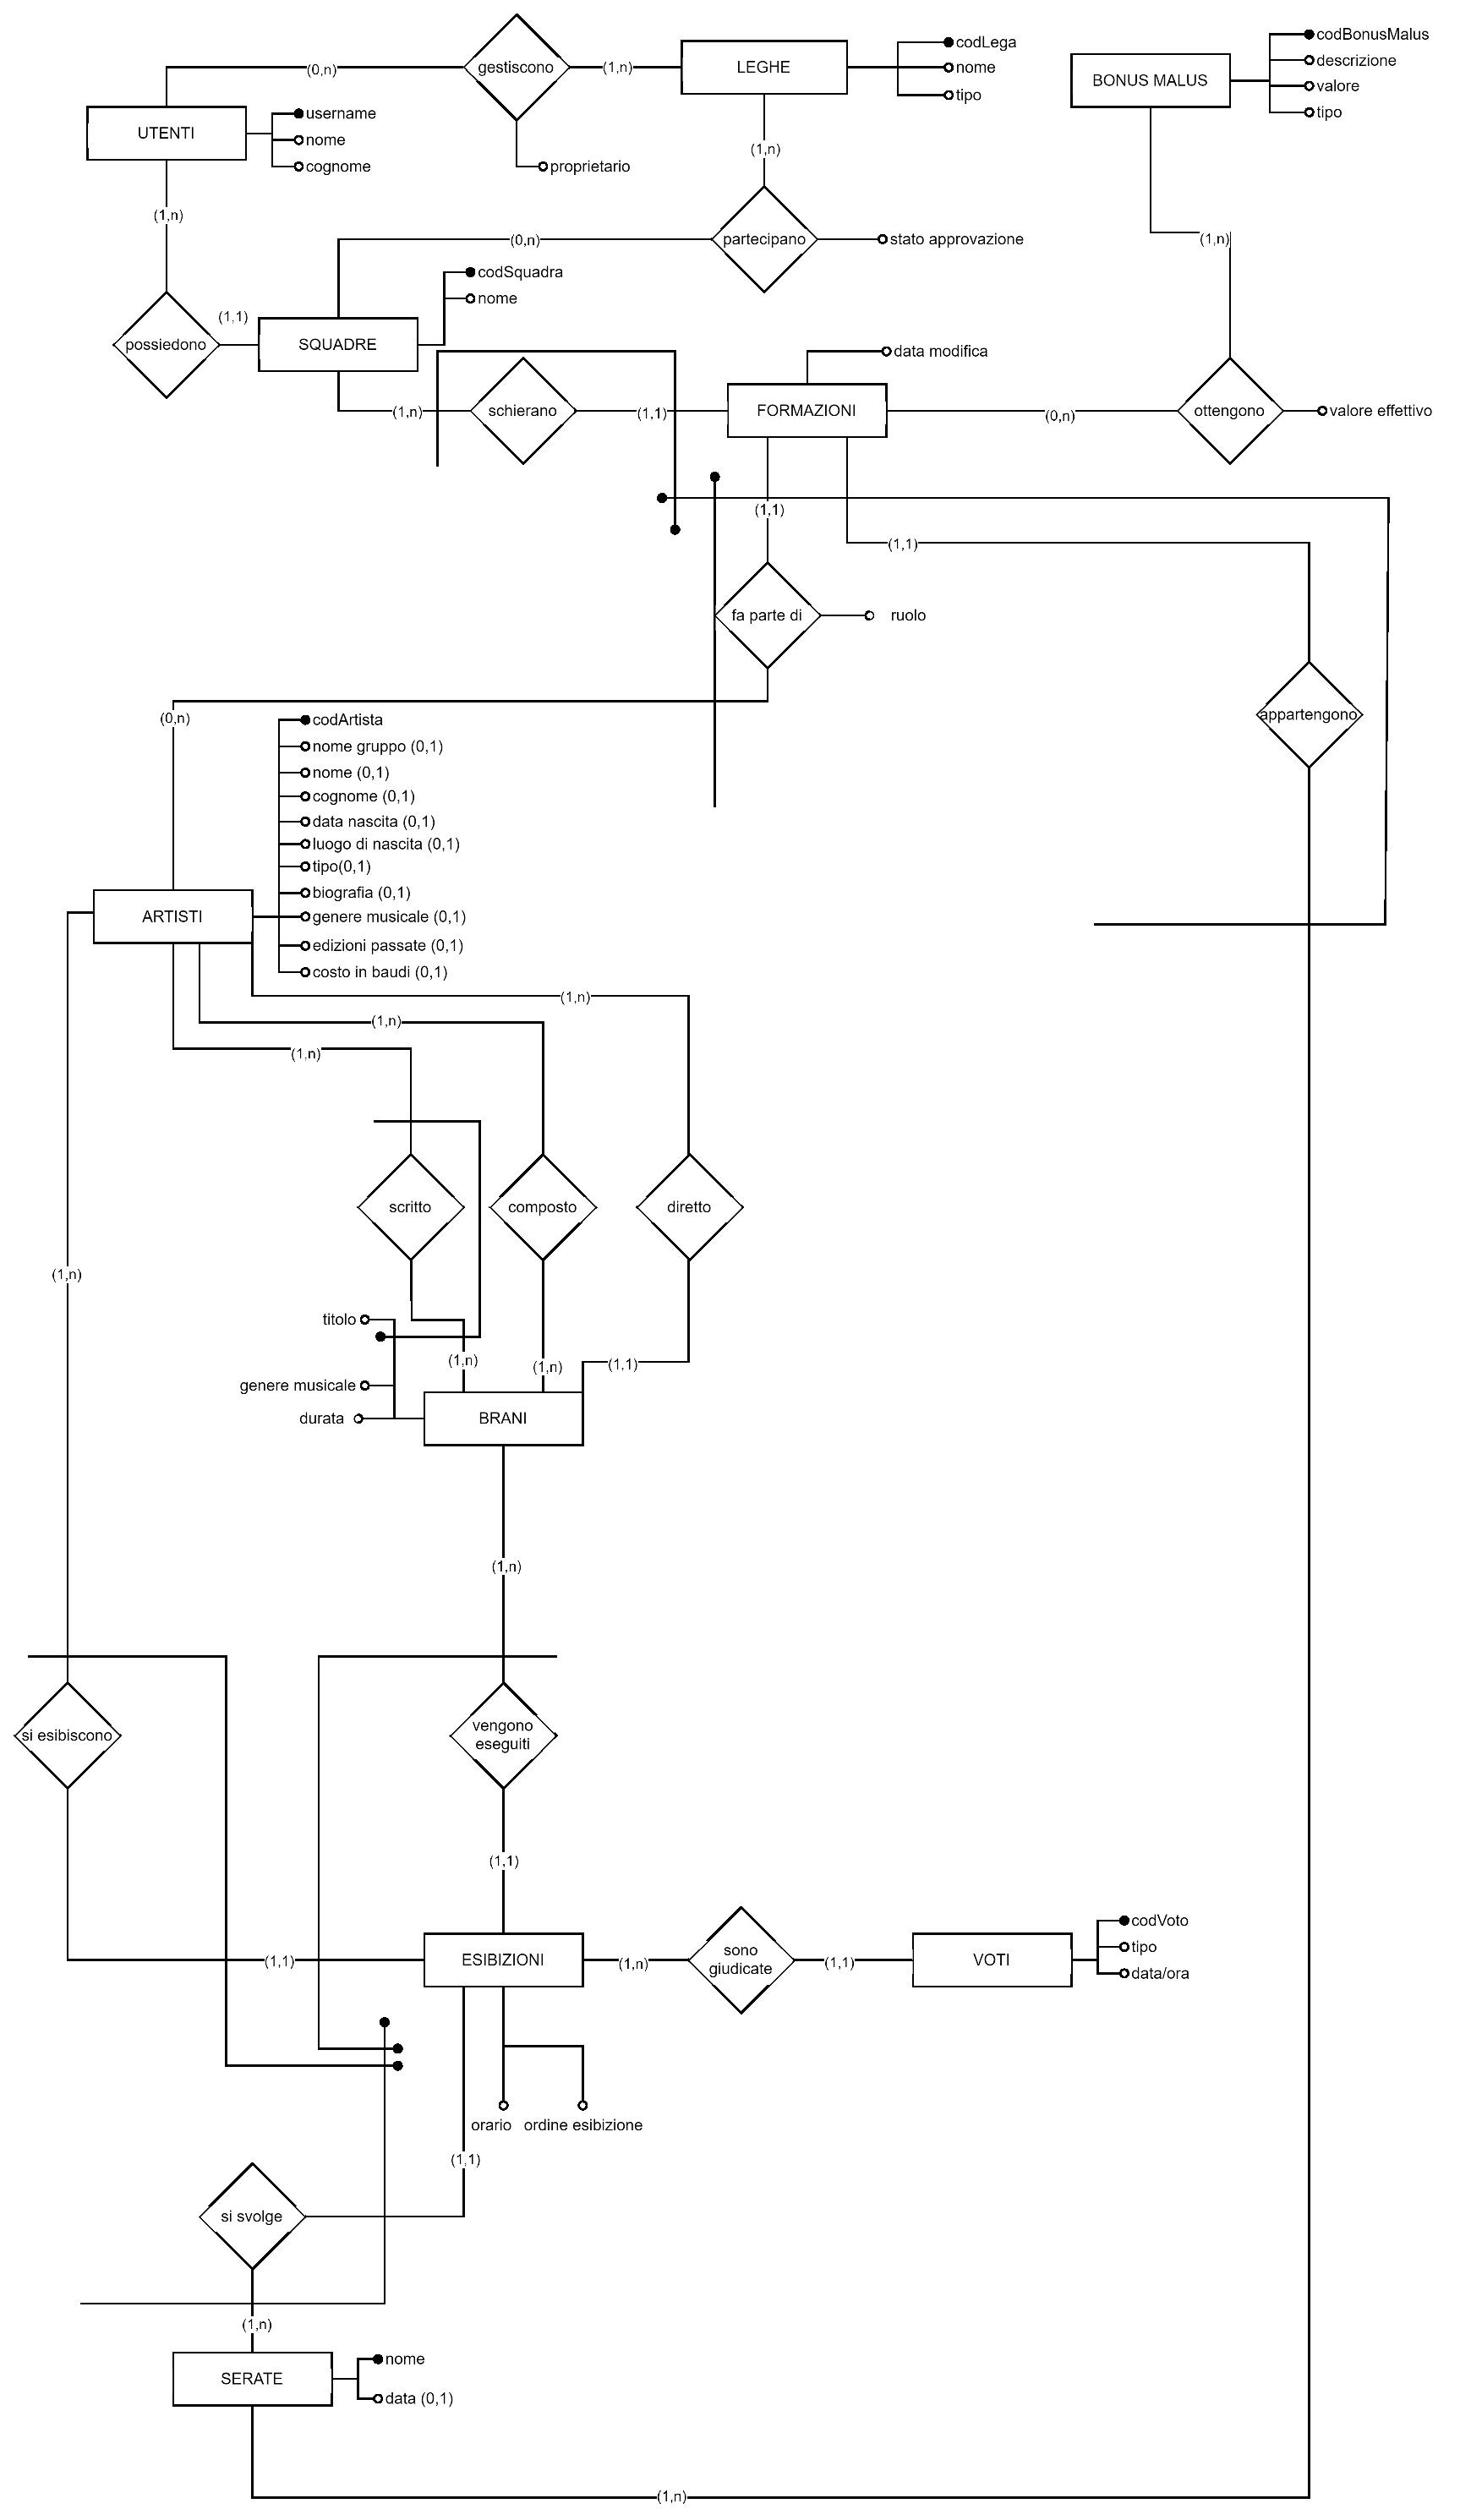
\includegraphics[width=0.8\textwidth]{schema_ER_ristrutturato.eps}
\end{center}

\subsection{Domini degli Attributi}
%[eventuali modifiche dei domini degli attributi e informazioni sui domini di eventuali attributi introdotti]
\begin{itemize}
	\item \textbf{(tipo, ARTISTI)} = tipo\_artista
	\begin{itemize}
		\item tipo\_artista = \{CANTANTE\}
	\end{itemize}
	\item \textbf{(tipo, CONTRIBUTI\_BRANI)} = ruolo\_artista
	\begin{itemize}
		\item ruolo\_artista = \{COMPOSITORE, DIRETTORE, SCRITTORE\}
	\end{itemize}
\end{itemize}

Per quanto riguarda i campi multi-valore è stato deciso di renderli un campo unico ed utilizzare la "," come carattere separatore (gestione lato software sapendo che verranno utilizzati di rado).


\subsection{Vincoli}
%[modifiche all'elenco di vincoli del modello concettuale (nuovi vincoli, eventuali vincoli eliminati o modificati)]
\begin{table}[h!]
	\centering
	\begin{tabular}{|c|c|p{6.5cm}|}
		\hline
		\textbf{Numero Vincolo} & \textbf{Entità e/o Associazioni Coinvolte} & \textbf{Vincolo in Linguaggio Naturale} \\ \hline
		1 & ARTISTI & Se un artista ha il tipo valorizzato a "C" (cantante), allora deve avere valorizzati gli attributi relativi al cantante: biografia, genere musicale, edizioni passate, costo in baudi. Viceversa, se almeno uno di questi attributi è valorizzato, allora il tipo deve essere "C".\\ \hline
	\end{tabular}
	\caption{Vincoli Non Esprimibili nel Diagramma ER}
\end{table}

\subsection{Ristrutturazione Gerarchie}
%[discussione delle scelte fatte per eliminare le gerarchie di generalizzazione]
L’unica gerarchia presente nello schema, quella tra ARTISTI e CANTANTI, è stata oggetto di ristrutturazione al fine di semplificare il modello. La gerarchia, parziale ed esclusiva, è stata rimossa e sostituita con un approccio basato su un attributo discriminante. In particolare, è stato introdotto l’attributo tipo nella relazione ARTISTI per distinguere gli artisti dai cantanti ("CANTANTE"). Gli attributi precedentemente associati a "CANTANTI" sono stati integrati come facoltativi direttamente in ARTISTI. Sebbene ciò comporti la presenza di valori nulli, si è ritenuta accettabile questa scelta in quanto la cardinalità della relazione è contenuta.

\subsection{Schema Logico}
%[schema logico relazionale nella notazione vista a lezione]
\begin{itemize}
	\item \textbf{UTENTI}(\underline{username}, nome, cognome)
	\item \textbf{LEGHE}(\underline{codLega}, nome, tipo)
	\item \textbf{BONUS\_MALUS}(\underline{codBonusMalus}, descrizione, valore, tipo)
	\item \textbf{SQUADRE}(\underline{codSquadra}, nome, username\textsuperscript{UTENTI})
	\item \textbf{FORMAZIONI}(\underline{codArtista}\textsuperscript{ARTISTI}, \underline{codSquadra}\textsuperscript{SQUADRE}, \underline{nomeSerata}\textsuperscript{SERATE}, ruolo, dataModifica)
	
	\item \textbf{GESTIONE\_LEGHE}(\underline{username}\textsuperscript{UTENTI}, \underline{codLega}\textsuperscript{LEGHE}, proprietario)
	\item \textbf{PARTECIPAZIONE\_LEGHE}(\underline{codSquadra}\textsuperscript{SQUADRE}, \underline{codLega}\textsuperscript{LEGHE}, statoApprovazione)
	\item \textbf{BONUS\_ASSEGNTI}(\underline{codSquadra}\textsuperscript{SQUADRE}, \underline{codArtista}\textsuperscript{ARTISTI}, \underline{nomeSerata}\textsuperscript{SERATE}, \underline{codBonusMalus}\textsuperscript{BONUS\_MALUS}, valoreEffettivo)
	
	\item \textbf{ARTISTI}(\underline{codArtista}, nomeGruppo\textsubscript{O}, nome\textsubscript{O}, cognome\textsubscript{O}, dataNascita\textsubscript{O}, luogoNascita\textsubscript{O}, tipo\textsubscript{O}, biografia\textsubscript{O}, genereMusicale\textsubscript{O}, edizioniPassate\textsubscript{O}, costoBaudi\textsubscript{O})
	\item \textbf{BRANI}(\underline{codBrano}, \uwave{titolo}, \uwave{codArtista}\textsuperscript{ARTISTI}, genereMusicale, durata)
	\item \textbf{SERATE}(\underline{nome}, data\textsubscript{O})
	\item \textbf{ESIBIZIONI}(\underline{codBrano}\textsuperscript{BRANI},\underline{codArtista}\textsuperscript{ARTISTI}, orario, ordineEsibizione, \underline{nomeSerata}\textsuperscript{SERATE})
	\item \textbf{VOTI}(\underline{codVoto}, codBrano\textsuperscript{BRANI}, codArtista\textsuperscript{ARTISTI}, nomeSerata\textsuperscript{SERATE}, tipo, dataOra)
	\item \textbf{CONTRIBUTI\_BRANI}(\underline{codBrano}\textsuperscript{BRANI}, \underline{codArtista}\textsuperscript{ARTISTI}, \underline{tipo})
\end{itemize}

\subsection{Verifica di Qualità dello Schema}
%[verifica delle forme normali ed eventuali ottimizzazioni applicate tenendo in considerazione il carico di lavoro]

\subsubsection{Dipendenze funzionali}

\begin{itemize}
	\item UTENTI: username → nome, cognome
	\item LEGHE: codLega → nome, tipo
	\item BONUS\_MALUS: codBonusMalus → descrizione, valore, tipo
	\item SQUADRE: codSquadra → nome, username
	\item FORMAZIONI: (codArtista, codSquadra, nomeSerata) → ruolo, dataModifica
	\item GESTIONE\_LEGHE: (username, codLega) → proprietario
	\item PARTECIPAZIONE\_LEGHE: (codSquadra, codLega) → statoApprovazione
	\item BONUS\_ASSEGNTI: (codSquadra, codArtista, nomeSerata, codBonusMalus) → valoreEffettivo
	\item ARTISTI: codArtista → nomeGruppo, nome, cognome, dataNascita,\\
	\hspace{4.5em} luogoNascita, tipo, biografia, genereMusicale, edizioniPassate, costoBaudi
	\item BRANI: codBrano → titolo, codArtista, genereMusicale, durata\\
	\hspace{4.5em}(codArtista, titolo) → codBrano, titolo, genereMusicale, durata
	\item SERATE: nome → data
	\item ESIBIZIONI: (codBrano, codArtista, nomeSerata) → orario, ordineEsibizione
	\item VOTI: codVoto → codBrano, codArtista, nomeSerata, tipo, dataOra
	\item CONTRIBUTI\_BRANI: (codBrano, codArtista) → tipo
\end{itemize}

\subsubsection{Verifica BCNF}
Tutte le relazioni presenti nello schema logico risultano essere in forma normale di Boyce-Codd (BCNF).  
Per ciascuna relazione, infatti, è stato verificato che ogni dipendenza funzionale non banale ha come determinante una superchiave.  
Questo garantisce un elevato livello di normalizzazione, con benefici in termini di assenza di ridondanze, integrità dei dati e semplificazione delle operazioni di aggiornamento.  
Non sono stati rilevati casi di violazione della BCNF, nemmeno in presenza di chiavi candidate alternative o vincoli condizionali, come nel caso della relazione \texttt{ARTISTI}.



\subsection{Schema SQL in Forma Grafica}
\begin{center}
	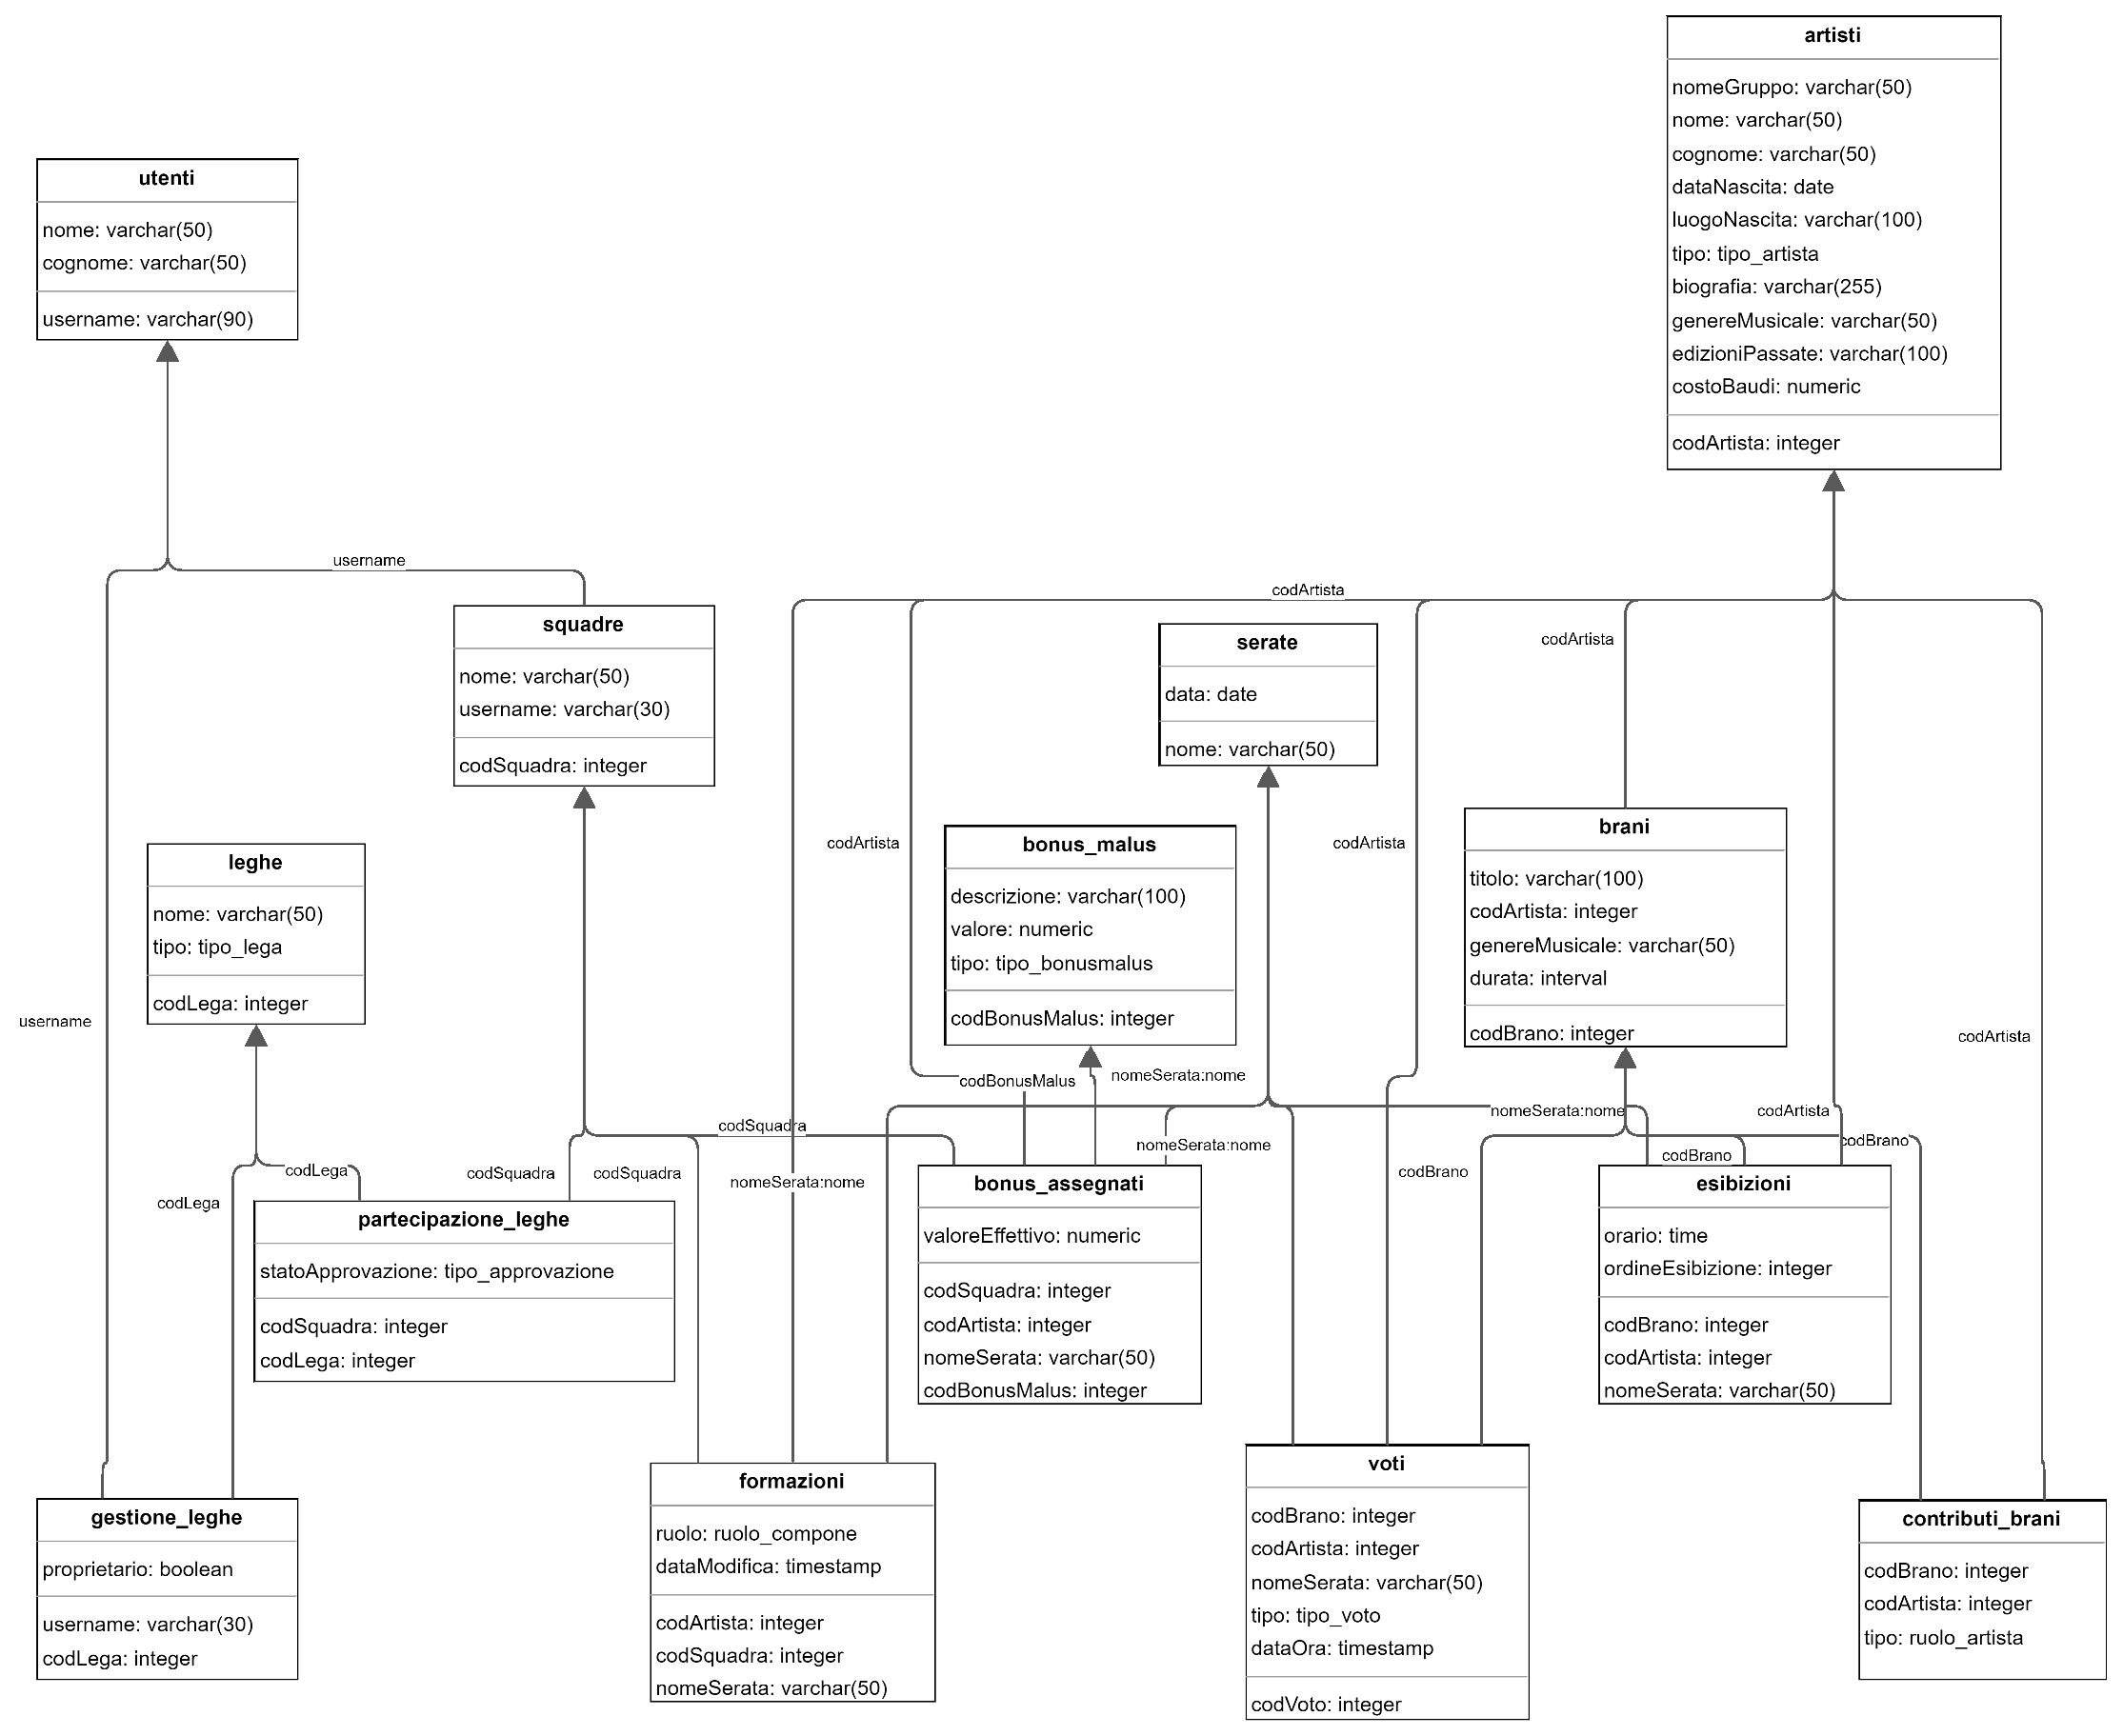
\includegraphics[width=0.9\textwidth]{fantasanremo.eps}
	%\caption{Diagramma dello schema relazionale generato con DataGrip}
\end{center}



\subsection{Uso di Intelligenza Artificiale Generativa}
%[Specificare se e come è stata utilizzata l’intelligenza artificiale generativa per realizzare le varie parti del progetto. Indicare anche se sono stati effettuati esperimenti di uso di AI generativa relativi al progetto che non hanno prodotto alcun contributo effettivamente utilizzato nel progetto consegnato, commentandone i risultati]
Nel corso dello sviluppo del presente progetto è stato fatto ricorso, in maniera mirata e controllata, a strumenti di intelligenza artificiale generativa, in particolare ChatGPT di OpenAI, con finalità esclusivamente assistive.\\
L’impiego dell’AI si è concentrato su alcune attività specifiche:
\begin{itemize}
	\item l’esplicitazione delle dipendenze funzionali a partire dallo schema logico relazionale;
	\item la verifica del rispetto delle forme normali, con particolare attenzione alla Boyce-Codd Normal Form (BCNF);
	\item il supporto alla redazione della documentazione in linguaggio \LaTeX;
	\item la definizione dei domini degli attributi, tramite l’impiego di tipi enumerati coerenti con la semantica del modello.
\end{itemize}

Tutti i contenuti generati con il supporto dell’intelligenza artificiale sono stati oggetto di verifica da parte dei componenti del gruppo, che hanno esercitato un controllo costante e consapevole sull’intero processo di progettazione. L’AI è stata dunque utilizzata esclusivamente come strumento di supporto operativo, e non come fonte automatica di soluzioni corrette in modo assoluto o prive di necessità di revisione critica.
\end{document}
